\documentclass[a4paper]{article}
\usepackage[utf8]{inputenc}
\usepackage[russian]{babel}
\usepackage[T2]{fontenc}
\usepackage[warn]{mathtext}
\usepackage{graphicx}
\usepackage{amsmath}
\usepackage{floatflt}
\usepackage[left=20mm, top=20mm, right=20mm, bottom=20mm, footskip=10mm]{geometry}


\graphicspath{ {images/} }
\usepackage{multicol}
\setlength{\columnsep}{2cm}


\begin{document}

\begin{titlepage}
	\centering
	\vspace{5cm}
	{\scshape\LARGE Московский физико-технический институт \par}
	\vspace{4cm}
	{\scshape\Large Лабораторная работа \par}
	\vspace{1cm}
	{\huge\bfseries Моделирование оптических приборов и определение их увеличения \par}
	\vspace{1cm}
	\vfill
\begin{flushright}
	{\large выполнила студент 653 группы ФФКЭ}\par
	\vspace{0.3cm}
	{\LARGE Давыдов Валентин} \par

\end{flushright}
	

	\vfill

% Bottom of the page
	Долгопрудный, 2018 г.
\end{titlepage}


\section{Цель работы:}
Определить фокусные расстояния собирающих и рассеивающих линз, смоделировать ход лучей в трубе Галилея, трубе Кеплера и микроскопе, определить их увеличение

\section{В работе используются:}
\begin{itemize}
    \item оптическая скамья
    \item набор линз
    \item экран
    \item осветитель со шкалой
    \item зрительная труба
    \item диафрагма
    \item линейка.
\end{itemize}

\section{Определение фокусных расстояний линз с помощью зрительной трубы}
\subsection{Определение фокусного расстояния собирающих линз}

\begin{enumerate}
    \item Настроим зрительную трубу на бесконечность
    \item Поставим положительную линзу на
расстоянии от предмета примерно равном фокусному. На небольшом расстоянии от линзы закрепим трубу, настроенную на бесконечность,
и отцентрируем её по высоте. Диафрагма диаметром
d = 1 см, надетая на ближнюю к осветителю линзу, уменьшит сферические аберрации и повысит чёткость изображения. \par
Передвигая линзу вдоль скамьи, получим в окуляре зрительной трубы изображение предмета
— миллиметровой сетки. При этом расстояние между предметом и серединой тонкой линзы (между проточками на оправах) равно фокусному.
    \item Результаты измерения фокусных расстояний собирающих линз:
    \begin{center}
        $f_1 = 11$ см \hspace{1cm}  $f_2 = 7.5$ см \hspace{1cm}  $f_3 = 25$ см
    \end{center}
\end{enumerate}

\subsection{Определение фокусного расстояния рассеивающих линз}
\begin{enumerate}
    \item Для определения фокусного расстояния тонкой отрицательной линзы сначала получим на экране увеличенное изображение сетки при помощи одной короткофокусной положительной линзы. Измерьте расстояние между линзой и экраном $a_0 = 30$ см.
    \item Разместите сразу за экраном трубу, настроенную на бесконечность, и закрепите её. Уберите экран и поставьте на его место исследуемую рассеивающую линзу (рис. 8). Перемещая рассеивающую линзу, найдите в окуляре зрительной трубы резкое изображение сетки. \par
    Измерив расстояние между линзами $l$, рассчитайте фокусное расстояние рассеивающей линзы $f = a_0 - l$.
    \item Результаты измерения фокусного расстояния рассеивающих линз:
    \begin{center}
        $f_1 = 2$ см \hspace{1cm}  $f_2 = 14$ см
    \end{center}
\end{enumerate}

\begin{figure}[h]
\begin{center}
\begin{minipage}[h]{0.40\linewidth}
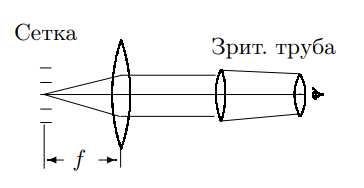
\includegraphics[width=1\linewidth]{plus_lens.PNG}
\caption{Определение фокусного расстояния собирающей линзы} %% подпись к рисунку
\label{ris:experimoriginal} %% метка рисунка для ссылки на него
\end{minipage}
\hfill 
\begin{minipage}[h]{0.40\linewidth}
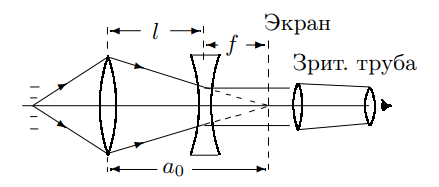
\includegraphics[width=1\linewidth]{minus_lens.PNG}
\caption{Определение фокусного расстояния рассеивающей линзы}
\label{ris:experimcoded}
\end{minipage}
\end{center}
\end{figure}

\section{Моделирование трубы Кеплера}
\begin{enumerate}
    \item Рассмотрим ход лучей в трубе Кеплера и найдём увеличение данной оптической системы:
    
    \begin{figure}[h]
    \centering
    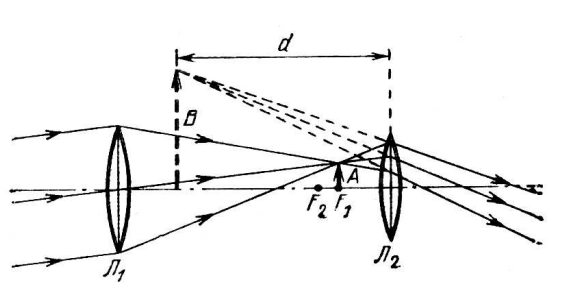
\includegraphics[width=9cm]{kepler.PNG}
    \caption{Ход лучей в трубе Кеплера}
    \label{fig:vac}
\end{figure}

Пусть пучок света, попадающий в объектив, составляет с оптической осью угол $\varphi_1$, а пучок, выходящий из окуляра, — угол $\varphi_2$. Увеличение $\gamma$ зрительной трубы по определению равно
\begin{equation}
    \gamma = \frac{\tan \varphi_2}{\tan \varphi_1},
\end{equation}
но также из рис. 3 следует, что 
\begin{equation}
    \gamma_K = \frac{f_1}{f_2} = \frac{D_1}{D_2},
\end{equation}
где $D_1$ - ширина пучка, прошедшего через объектив, а $D_2$ - ширина пучка, вышедшего из окуляра

\item Построим оптическую систему из каллиматора и непосредственно трубы Кеплера. 

    \begin{figure}[h]
    \centering
    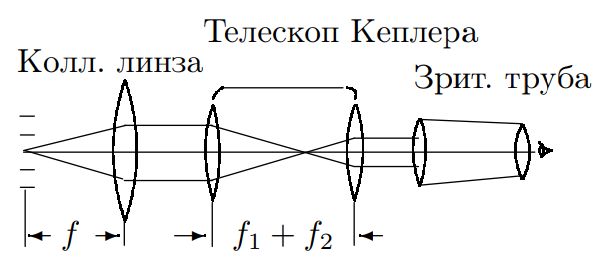
\includegraphics[width=9cm]{kepler_2.PNG}
    \caption{Схема трубы Кеплера}
    \label{fig:vac}
\end{figure}

Параметры действующих линз:
\begin{center}
    $f_1 = 25$ см \hspace{1cm} $f_2 = 13$ см
\end{center}

Найдём увеличение трубы Кеплера непосредственно: пусть $h_1$ - размер ячейки миллиметровой сетки без телескопа, $h_2$ - с телескопом
\begin{center}
$h_1 = 1.5$ дел., \hspace{1cm} $h_2 = 2.8$ дел. \par
$\gamma_K = \frac{h_2}{h_1} = 1.867$
\end{center}

При этом по формуле (2) также
\begin{center}
    $\gamma_K = \frac{f_1}{f_2} = 1.923$
\end{center}

Полученные значения практически совпадают
\end{enumerate}

\section{Моделирование трубы Галилея}
    \begin{figure}[h]
    \centering
    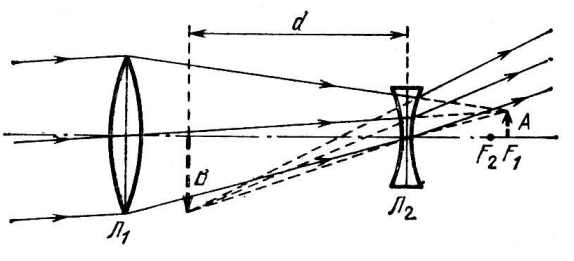
\includegraphics[width=9cm]{gal.PNG}
    \caption{Ход лучей в трубе Галилея}
    \label{fig:vac}
\end{figure}

\begin{enumerate}
    \item Труба Галилея получается из трубы Кеплера заменой собирающей линзы окуляра рассеивающей. Формулы для увеличения, соответственно, остаются теми же:
\begin{equation}
    \gamma_G = \frac{f_1}{f_2} = \frac{D_1}{D_2},
\end{equation}

\item Заменим собирающую линзу с фокусным расстоянием $f_2 = 13$ см рассеивающей с фокусным расстоянием $f_2 = 14$ см. Проведём те же операции, что и для трубы Кеплера:

\begin{center}
$h_1 = 1.5$ дел., \hspace{1cm} $h_2 = 2.6$ дел. \par
$\gamma_K = \frac{h_2}{h_1} = 1.733$
\end{center}

При этом по формуле (2) также
\begin{center}
    $\gamma_K = \frac{f_1}{f_2} = 1.786$
\end{center}

Полученные значения практически совпадают.
\end{enumerate}

\section{Моделирование микроскопа}

    \begin{figure}[h]
    \centering
    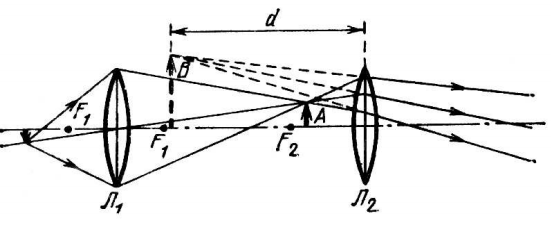
\includegraphics[width=9cm]{micro.PNG}
    \caption{Ход лучей в микроскопе}
    \label{fig:vac}
\end{figure}

\begin{enumerate}
    \item Ход лучей в микроскопе показан на рис. 6. Увеличение микроскопа вычисляется по формуле
    \begin{equation}
        \gamma_M = \Gamma_o_b \Gamma_o_c = \frac{\triangle}{f_1} \frac{L}{f_2},
    \end{equation}
    где $f_1$ и $f_2$ - фокусные расстояния линз микроскопа, $\triangle = 16$ см - длина тубуса, $L$ - расстояние наилучшего зрения ($L = 25$ см).
    
    \begin{figure}[h]
    \centering
    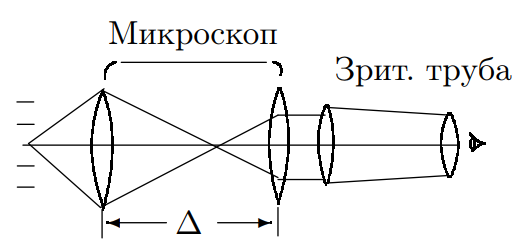
\includegraphics[width=9cm]{micro_2.PNG}
    \caption{Схема микроскопа}
    \label{fig:vac}
\end{figure}    
    
    \item Соберём микроскоп с пятикратным увеличением. Используемые линзы: $f_1 = 11$ см, $f_2 = 7.5$ см. Получим
    \begin{center}
        $\gamma_M = \frac{\triangle}{f_1} \frac{L}{f_2} = 4.848$ \par
        $\gamma_M = \frac{h_2}{h_1} = \frac{7.2}{1.5} = 4.8$
    \end{center}
Значения практически совпадают
\end{enumerate}

\section{Вывод}
В ходе работы были определены фокусные расстояния собирающих и рассеивающих линз с помощью зрительной трубы. Из этих линз далее сконструированы следующие оптические приборы: труба Кеплера, труба Галилея, микроскоп. Были определены их увеличения и проведено сравнение с её действительным значением:

\begin{center}
    $\gamma_K_t_h = 1.923$ \hspace{1cm} $\gamma_K_e_x = 1.867$ \par \vspace{1cm} 
    $\gamma_G_t_h = 1.786$ \hspace{1cm} $\gamma_G_e_x = 1.733$ \par \vspace{1cm}  
    $\gamma_M_t_h = 4.848$ \hspace{1cm} $\gamma_M_e_x = 4.800$ 
    \end{center}
    
\end{document}
